% !TEX program = xelatex
% Báo cáo chi tiết YC1 — Training & Evaluation ECAPA-TDNN
% Compile: xelatex training_report.tex  (chạy 2-3 lần để có mục lục + tham chiếu)
\documentclass[12pt,a4paper]{article}

\usepackage{fontspec}
\setmainfont{Latin Modern Roman}
\setmonofont{Latin Modern Mono}

\usepackage{geometry}
\geometry{margin=2.4cm}
\usepackage{booktabs}
\usepackage{longtable}
\usepackage{array}
\usepackage{enumitem}
\usepackage{xcolor}
\usepackage{amsmath}
\usepackage{amssymb}
\usepackage{graphicx}
\usepackage{float}
\usepackage{caption}
\usepackage[most]{tcolorbox}
\usepackage{tikz}
\usetikzlibrary{arrows.meta, positioning, shapes.geometric, fit, calc}
\usepackage{listings}
\usepackage{hyperref}

\definecolor{accent}{HTML}{1D4ED8}
\hypersetup{colorlinks=true, linkcolor=accent, urlcolor=accent, citecolor=accent,
  pdftitle={Bao cao chi tiet YC1 - Training ECAPA-TDNN}, pdfauthor={Secure-VA}}
\setlist[itemize]{leftmargin=1.2cm,topsep=2pt,itemsep=1pt}
\setlist[enumerate]{leftmargin=1.2cm,topsep=2pt,itemsep=1pt}
\renewcommand{\arraystretch}{1.25}
\captionsetup{font=small,labelfont=bf}

% ---------- Callout boxes (theo style báo cáo YC2) ----------
\newtcolorbox{diembox}[1][Điểm chính]{enhanced,breakable,colback=green!4,
  colframe=green!45!black,coltitle=white,fonttitle=\bfseries\small,title={#1},
  boxrule=0.6pt,left=4pt,right=4pt,top=3pt,bottom=3pt,arc=2pt}
\newtcolorbox{luuybox}[1][Lưu ý]{enhanced,breakable,colback=orange!5,
  colframe=orange!65!black,coltitle=white,fonttitle=\bfseries\small,title={#1},
  boxrule=0.6pt,left=4pt,right=4pt,top=3pt,bottom=3pt,arc=2pt}
\newtcolorbox{ycbox}[1][Ý chính khi giải thích code]{enhanced,breakable,colback=blue!4,
  colframe=blue!55!black,coltitle=white,fonttitle=\bfseries\small,title={#1},
  boxrule=0.6pt,left=4pt,right=4pt,top=3pt,bottom=3pt,arc=2pt}

% ---------- Code style ----------
\lstdefinestyle{py}{language=Python,basicstyle=\ttfamily\scriptsize,
  keywordstyle=\color{blue!60!black},commentstyle=\color{green!45!black}\itshape,
  stringstyle=\color{orange!70!black},breaklines=true,frame=single,
  columns=fullflexible,backgroundcolor=\color{gray!6},keepspaces=true,
  showstringspaces=false,numbers=none,xleftmargin=4pt,framexleftmargin=4pt}
\lstset{style=py}

% ---------- TikZ node styles ----------
\tikzset{
  io/.style={rectangle,rounded corners=2pt,draw=blue!55!black,fill=blue!6,
    align=center,font=\footnotesize,inner sep=4pt,minimum height=8mm},
  proc/.style={rectangle,rounded corners=2pt,draw=teal!60!black,fill=teal!8,
    align=center,font=\footnotesize,inner sep=4pt,minimum height=8mm},
  loss/.style={rectangle,rounded corners=2pt,draw=red!55!black,fill=red!6,
    align=center,font=\footnotesize,inner sep=4pt,minimum height=8mm},
  ar/.style={-{Stealth[length=2mm]},thick,draw=black!70}
}

\title{\textbf{Báo cáo chi tiết YC1}\\[4pt]
\large Huấn luyện \& Đánh giá Mô hình Nhận dạng Người nói (ECAPA-TDNN)}
\author{Đồ án: Secure Virtual Assistant with Speaker Recognition}
\date{Tháng 6, 2026}

\begin{document}
\maketitle

\begin{tcolorbox}[enhanced,colback=blue!3,colframe=blue!40!black,arc=3pt,
  boxrule=0.5pt,left=6pt,right=6pt]
\textbf{Phạm vi:} Báo cáo tập trung vào Yêu cầu 1 (YC1) --- \emph{huấn luyện và
đánh giá} mô hình ECAPA-TDNN cho Speaker Identification (SID) và Speaker
Verification (SV). Trình bày chi tiết \emph{từng bước} với \emph{trích đoạn code
thật} kèm giải thích, sơ đồ, công thức và bộ kết quả thực nghiệm trên hai dataset
\emph{VoxCeleb Indian} và \emph{VIVOS}. Không đi sâu vào tầng bảo mật/ứng dụng
(YC2) ngoài cách runtime sử dụng SID/SV score. Tài liệu viết bằng tiếng Việt.
\end{tcolorbox}

\tableofcontents
\newpage

% ============================================================
\section{Mục tiêu của YC1}
% ============================================================
YC1 trả lời hai câu hỏi nền tảng của trợ lý ảo có giọng nói:

\begin{itemize}
  \item \textbf{Ai đang nói?} --- \textbf{Speaker Identification (SID)}: phân loại
  giọng nói vào một trong $N$ người đã đăng ký (closed-set, multi-class).
  \item \textbf{Có đúng là người đó không?} --- \textbf{Speaker Verification (SV)}:
  quyết định nhị phân chấp nhận/từ chối khi so giọng hiện tại với một người cụ thể.
\end{itemize}

\begin{diembox}[Tư tưởng cốt lõi]
Hệ thống dùng \textbf{một mô hình embedding duy nhất} cho cả hai bài toán: huấn
luyện theo kiểu \emph{phân loại người nói} (speaker classification), sau đó lấy
vector embedding 192 chiều và so khớp bằng \textbf{cosine similarity}. SID chọn
người có cosine cao nhất; SV so cosine với một ngưỡng. Đây là chuẩn của các hệ
thống speaker recognition hiện đại.
\end{diembox}

% ============================================================
\section{Các file cần đọc trong phần training}
% ============================================================
\begin{table}[H]
\centering
\small
\begin{tabular}{p{0.27\linewidth}p{0.66\linewidth}}
\toprule
\textbf{File} & \textbf{Vai trò trong YC1} \\
\midrule
\texttt{training/train\_ecapa.py} & Toàn bộ logic train: Dataset, tiền xử lý, mel,
ECAPA-TDNN, AAM-Softmax, vòng lặp train/val, lưu checkpoint. \\
\texttt{training/evaluate\_sid.py} & Đánh giá SID: Top-1/Top-5, và (bản nâng cấp)
micro/macro/weighted-F1 + confusion matrix. \\
\texttt{training/evaluate\_sv.py} & Đánh giá SV: EER, minDCF, threshold; (bản nâng
cấp) lưu (label, score) để vẽ DET/ROC. \\
\texttt{training/augmentations.py} & Khung augmentation tùy chọn: speed, MUSAN
noise, RIR reverb, SpecAugment. \\
\texttt{notebooks/SecureVA-V*.ipynb} & Ba vòng thực nghiệm trên
Kaggle; V3 sinh evidence chính thức. \\
\texttt{results/<dataset>/} & Artifact: checkpoint, log, split, kết quả
SID/SV, hparams. \\
\bottomrule
\end{tabular}
\caption{Bản đồ đọc code cho phần huấn luyện.}
\end{table}

% ============================================================
\section{Bức tranh tổng thể: pipeline huấn luyện và suy luận}
% ============================================================
Quá trình gồm hai giai đoạn dùng \emph{chung} mạng ECAPA-TDNN.

\begin{figure}[H]
\centering
\begin{tikzpicture}[node distance=8mm and 9mm]
\node[io] (a) {Audio\\.wav};
\node[proc,right=of a] (p) {Tiền xử lý\\16kHz, mono\\crop 3s};
\node[proc,right=of p] (m) {Mel 80-d\\log + CMN};
\node[proc,right=of m] (e) {ECAPA-TDNN\\emb 192-d};
\node[loss,right=of e] (l) {AAM-Softmax\\loss};
\draw[ar] (a)--(p); \draw[ar] (p)--(m); \draw[ar] (m)--(e); \draw[ar] (e)--(l);
\node[below=1mm of e,font=\scriptsize\itshape,text=teal!50!black] {(L2-normalize)};
\end{tikzpicture}
\caption{Giai đoạn HUẤN LUYỆN: tối ưu cross-entropy có biên góc trên nhãn người nói.}
\end{figure}

\begin{figure}[H]
\centering
\begin{tikzpicture}[node distance=7mm and 10mm]
\node[io] (a) {Audio\\mới};
\node[proc,right=of a] (e) {ECAPA\\$\to$ emb $x$};
\node[io,right=2.4cm of e,yshift=9mm] (sid) {\textbf{SID}: $\arg\max_i \cos(x,W_i)$\\$\to$ người + margin};
\node[io,right=2.4cm of e,yshift=-9mm] (sv) {\textbf{SV}: $\cos(x,c_{user})\ge\tau$\\$\to$ accept/reject};
\draw[ar] (a)--(e);
\draw[ar] (e.east) to[out=20,in=180] (sid.west);
\draw[ar] (e.east) to[out=-20,in=180] (sv.west);
\end{tikzpicture}
\caption{Giai đoạn SUY LUẬN: cùng embedding $x$ phục vụ cả SID (so với trọng số
lớp/centroid) và SV (so với centroid của 1 user theo ngưỡng $\tau$).}
\end{figure}

\begin{diembox}[Câu nên nói khi vấn đáp]
Mô hình \emph{không} được train trực tiếp cho SV. Nó được train để \emph{phân loại}
người nói; chính quá trình đó ép embedding của cùng một người xích lại gần nhau và
khác người thì tách xa --- nhờ vậy cosine giữa hai embedding trở thành thước đo
``cùng người hay không''.
\end{diembox}

% ============================================================
\section{Dữ liệu và cách chia tập}
% ============================================================
\subsection{Hai bộ dữ liệu}
\begin{table}[H]
\centering\small
\begin{tabular}{lrrrrrr}
\toprule
\textbf{Dataset} & \textbf{Spk} & \textbf{Utt} & \textbf{Train} & \textbf{Val} & \textbf{Test} & \textbf{Trial SV} \\
\midrule
VoxCeleb Indian & 24 & 4{,}857 & 3{,}389 & 717 & 751 & 552 \\
VIVOS & 65 & 12{,}419 & 8{,}686 & 1{,}850 & 1{,}883 & 4{,}160 \\
\bottomrule
\end{tabular}
\caption{Thống kê (seed = 42). VIVOS gộp 46 speaker tập train + 19 speaker tập test.}
\end{table}

\subsection{Vì sao chọn hai dataset này?}
Việc chọn dataset bám theo \emph{mục tiêu sử dụng} (trợ lý ảo tiếng Việt) và
\emph{ràng buộc tài nguyên} (train miễn phí trên Kaggle GPU). Lý do cụ thể:

\begin{itemize}
  \item \textbf{VIVOS --- dataset chính:}
  \begin{itemize}
    \item \emph{Đúng miền tiếng Việt}: người dùng thật nói tiếng Việt; model train
    trên giọng Việt sẽ không bị lệch miền khi deploy.
    \item \emph{Đủ lớn cho closed-set}: 65 người $\times$ ~12k câu --- đủ để học
    embedding phân biệt mà vẫn train được trong vài giờ trên 1 GPU.
    \item \emph{Sạch, gán nhãn rõ}: là corpus ASR tiếng Việt chuẩn (ĐH KHTN),
    nhãn speaker tin cậy, license học thuật rõ ràng.
    \item \emph{Miễn phí, có sẵn trên Kaggle} → tái lập dễ.
  \end{itemize}
  \item \textbf{VoxCeleb Indian subset --- dataset đối chứng:}
  \begin{itemize}
    \item \emph{Kiểm chứng tính tổng quát}: audio YouTube ``in-the-wild'' (nhiễu,
    đa micro, đa môi trường) --- chứng minh pipeline không chỉ chạy tốt trên dữ
    liệu sạch.
    \item \emph{Là chuẩn học thuật}: VoxCeleb là benchmark speaker recognition phổ
    biến nhất → kết quả dễ đối chiếu với văn liệu.
    \item \emph{Subset Indian nhỏ gọn} (24 người): vừa đủ tài nguyên Kaggle, không
    cần tải VoxCeleb full (hàng trăm GB).
  \end{itemize}
\end{itemize}

\begin{diembox}[Tóm tắt lý do chọn dataset]
VIVOS để \textbf{khớp miền} (tiếng Việt, sạch, đúng đối tượng người dùng);
VoxCeleb Indian để \textbf{đối chứng độ bền} trên dữ liệu nhiễu thực tế. Cả hai
đều \emph{miễn phí + có trên Kaggle} nên train lại được, và \emph{đủ nhỏ} để vừa
tài nguyên GPU free-tier.
\end{diembox}

\subsection{Quá trình chuẩn bị dataset (5 bước)}
Toàn bộ khâu chuẩn bị nằm trong notebook \texttt{SecureVA-V3.ipynb}, gồm 5 bước:

\begin{enumerate}
  \item \textbf{Tải \& gom dữ liệu}: add dataset trên Kaggle; với VIVOS, gộp
  \texttt{train/} và \texttt{test/} vào một thư mục \texttt{vivos\_speaker\_root}
  để có đủ 65 speaker trong một closed-set.
  \item \textbf{Quét file \& loại audio lỗi}: duyệt từng \texttt{.wav}, thử
  \texttt{torchaudio.load}; file hỏng bị ghi vào \texttt{bad\_audio\_files.txt} và
  loại khỏi split (VIVOS: 1 file). Chỉ giữ speaker có $\ge 3$ utterance để chia
  được cả 3 tập.
  \item \textbf{Chia split phân tầng theo speaker} (70/15/15) --- xem Mục~4.4.
  \item \textbf{Sinh trial pair SV} (cân bằng dương/âm) --- xem Mục~4.5.
  \item \textbf{Dump thống kê}: ghi \texttt{dataset\_summary.json} (số speaker,
  utterance, kích thước split, số trial) để kiểm tra và đưa vào báo cáo.
\end{enumerate}

\subsection{Tạo split phân tầng theo từng người nói}
Mỗi người nói được xáo trộn \emph{riêng} rồi chia 70/15/15, đảm bảo \emph{mọi
speaker đều xuất hiện ở cả ba tập} --- đúng định nghĩa closed-set SID.

\begin{lstlisting}
for spk, files in spk2files.items():
    random.shuffle(files)                 # xao tron rieng tung speaker
    n = len(files)
    n_train = max(1, int(0.70 * n)); n_val = max(1, int(0.15 * n))
    train, val, test = files[:n_train], files[n_train:n_train+n_val], files[n_train+n_val:]
    for p in train: iden_lines.append(f"1 {p}\n")   # 1 = train
    for p in val:   iden_lines.append(f"2 {p}\n")   # 2 = val
    for p in test:  iden_lines.append(f"3 {p}\n")   # 3 = test
\end{lstlisting}

\textbf{Giải thích:} file \texttt{iden\_split.txt} là ``mục lục'' của dataset; mỗi
dòng gồm mã split (1/2/3) và đường dẫn tương đối. \texttt{train\_ecapa.py} chỉ đọc
các dòng đúng split cần dùng. Cách chia theo speaker (thay vì trộn toàn cục) tránh
việc một người vắng mặt khỏi tập train.

\subsection{Sinh trial pair cho SV}
SV cần các \emph{cặp thử}: nhãn 1 (cùng người) hoặc 0 (khác người), số cặp dương/âm
được cân bằng.

\begin{lstlisting}
# Cap duong: ghep cac file CUNG mot nguoi (gioi han 3 cap/file de khong bung no)
for files in test_by_spk.values():
    for i in range(len(files)):
        for j in range(i+1, min(i+4, len(files))):
            pos.append((1, files[i], files[j]))
# Cap am: ghep file cua HAI nguoi khac nhau
for i in range(len(spks)):
    for j in range(i+1, len(spks)):
        neg.append((0, random.choice(test_by_spk[spks[i]]), random.choice(test_by_spk[spks[j]])))
k = min(len(pos), len(neg)); trials = random.sample(pos, k) + random.sample(neg, k)
\end{lstlisting}

\textbf{Giải thích các lựa chọn:} (i) \emph{cap 3 cặp dương/file} tránh bùng nổ số
cặp khi một người có nhiều câu (tổ hợp $C^2_n$ rất lớn); (ii) \emph{cân bằng
dương/âm} ($k=\min$) để EER không bị lệch về một phía; (iii) chọn 70/15/15 là tỉ
lệ phổ biến --- đủ dữ liệu train, vẫn còn val để chọn checkpoint và test để báo cáo.

\begin{luuybox}[Caveat về dữ liệu --- cần nói rõ khi vấn đáp]
\textbf{(1) Rò rỉ phiên:} split phân tầng theo speaker nhưng \emph{không} nhóm theo
\texttt{video\_id} (phiên YouTube) $\Rightarrow$ utterance cùng phiên có thể nằm cả
train lẫn test, khiến chỉ số \emph{lạc quan hơn} thực tế. Đây \textbf{không phải}
bộ VoxCeleb1-O chính thức.\\
\textbf{(2) Trial nhỏ (VoxCeleb):} 552 cặp $\to$ EER có sai số thống kê rộng
($\sim\!\pm2\%$).\\
\textbf{(3) Lệch miền:} VoxCeleb Indian là giọng Ấn (in-the-wild, nhiễu); VIVOS là
giọng đọc sạch --- dễ hơn hội thoại thực.
\end{luuybox}

% ============================================================
\section{Tiền xử lý chi tiết}
% ============================================================
Đây là phần ``làm gì với audio trước khi vào mạng''. Cài đặt ở
\texttt{VoxCelebSID.\_load} và \texttt{FbankExtractor}.

\subsection{Chuẩn hoá waveform: resample, mono, cắt/đệm 3 giây}
\begin{lstlisting}
wav, sr = torchaudio.load(str(path))
if sr != self.sample_rate:                       # (1) dua ve 16 kHz
    wav = torchaudio.functional.resample(wav, sr, self.sample_rate)
wav = wav.mean(dim=0)                             # (2) tron stereo -> mono
if wav.size(0) >= self.num_samples:               # (3) cat ve dung 3s
    if self.split == "train":
        start = random.randint(0, wav.size(0) - self.num_samples)   # random crop
    else:
        start = (wav.size(0) - self.num_samples) // 2               # center crop
    wav = wav[start:start + self.num_samples]
else:
    wav = F.pad(wav, (0, self.num_samples - wav.size(0)))           # zero-pad neu ngan
\end{lstlisting}

\textbf{Giải thích từng bước:}
\begin{enumerate}
  \item \textbf{Resample 16 kHz}: thống nhất tần số lấy mẫu --- ECAPA và mel-filter
  đều giả định 16 kHz.
  \item \textbf{Mono}: lấy trung bình kênh, vì danh tính người nói không phụ thuộc
  số kênh.
  \item \textbf{Cắt 3 giây} ($48{,}000$ mẫu): khi train dùng \emph{random crop} ---
  mỗi epoch thấy một đoạn khác nhau, đóng vai trò augmentation thời gian \emph{miễn
  phí}; khi eval dùng \emph{center crop} để kết quả tái lập. Audio ngắn hơn 3s thì
  \emph{zero-pad} ở cuối.
\end{enumerate}

\begin{ycbox}[Vì sao random vs center crop?]
Random crop lúc train giúp mô hình không học thuộc một đoạn cố định, tăng tính
tổng quát. Center crop lúc eval khử yếu tố ngẫu nhiên để hai lần chạy ra cùng số.
Khi \emph{trích embedding lúc deploy}, hệ thống dùng \emph{toàn bộ utterance} (không
crop) để embedding ổn định nhất.
\end{ycbox}

\subsection{Trích đặc trưng Mel-filterbank + log + CMN}
\begin{lstlisting}
self.mel = torchaudio.transforms.MelSpectrogram(
    sample_rate=16000, n_fft=512, win_length=400,   # 25 ms
    hop_length=160, n_mels=80)                       # 10 ms hop, 80 bins
def forward(self, x):
    m = self.mel(x)                 # pho Mel
    m = torch.log(m + 1e-6)         # nen dai dong (log)
    m = m - m.mean(dim=-1, keepdim=True)   # CMN: tru trung binh theo thoi gian
    return m.transpose(1, 2)        # -> [B, T, 80] cho ECAPA
\end{lstlisting}

\textbf{Giải thích:} mỗi 10 ms sinh một khung 80 chiều mô tả năng lượng theo dải
tần Mel (gần với cảm nhận tai người). Hai phép hậu xử lý quan trọng:
\begin{itemize}
  \item \textbf{Log}: $\log(\text{mel}+10^{-6})$ nén dải động (biên độ chênh lệch
  lớn) về thang dễ học; $10^{-6}$ tránh $\log 0$.
  \item \textbf{CMN (Cepstral Mean Normalization)}: trừ trung bình theo trục thời
  gian, $m' = m - \overline{m}_t$. Loại thiên lệch do \emph{kênh truyền/micro} ---
  giúp embedding bền hơn khi đổi thiết bị thu.
\end{itemize}

\subsection{Augmentation tuỳ chọn (đã có khung, mặc định tắt)}
\texttt{augmentations.py} cung cấp pipeline chỉ chạy khi train. Ví dụ trộn nhiễu
MUSAN theo SNR mục tiêu:
\begin{lstlisting}
def _mix_noise(self, wav):
    noise = _fit_length(_load_mono(random.choice(self.musan_files), sr), wav.numel())
    snr = random.uniform(*self.snr_db)                       # vd 5..20 dB
    scale = torch.sqrt(clean_power / (noise_power * 10 ** (snr/10)))
    return wav + scale * noise                               # tron theo SNR
\end{lstlisting}
Ngoài ra có \textbf{speed perturb} (0.9/1.0/1.1$\times$), \textbf{RIR reverb}
(tích chập đáp ứng phòng) và \textbf{SpecAugment} (che ngẫu nhiên dải tần/thời gian
trên log-mel).

\begin{luuybox}[Trạng thái trong evidence]
Trong các kết quả của báo cáo này, augmentation \textbf{tắt} (\texttt{augment=false}
trong \texttt{hparams.json}) do môi trường Kaggle chưa có dataset MUSAN/RIR hợp lệ.
Đây là một hướng cải tiến đã sẵn khung (xem Mục~\ref{sec:future}).
\end{luuybox}

% ============================================================
\section{Kiến trúc mô hình và hàm mất mát}
% ============================================================
\subsection{ECAPA-TDNN}
\begin{lstlisting}
model = ECAPA_TDNN(input_size=80, lin_neurons=192,
                   channels=[512, 512, 512, 512, 1536])   # ~6.2M params
\end{lstlisting}
ECAPA-TDNN (Desplanques 2020) là baseline state-of-the-art cho speaker embedding:
dùng \emph{SE-Res2Block} (chú ý kênh), \emph{multi-layer feature aggregation} và
\emph{attentive statistics pooling} để gộp toàn bộ utterance thành một vector 192
chiều. Dùng cài đặt SpeechBrain để khỏi ``phát minh lại bánh xe''.

\subsection{AAM-Softmax (Additive Angular Margin)}
\begin{lstlisting}
def forward(self, embeddings, labels):
    emb_n = F.normalize(embeddings, dim=1); w_n = F.normalize(self.weight, dim=1)
    cos_theta = F.linear(emb_n, w_n).clamp(-1+1e-7, 1-1e-7)   # cos goc emb<->lop
    theta = torch.acos(cos_theta)
    target = F.one_hot(labels, cos_theta.size(1)).bool()
    theta_m = torch.where(target, theta + self.margin, theta) # cong bien vao lop dung
    logits = self.scale * torch.cos(theta_m)                  # margin=0.2, scale=30
    return F.cross_entropy(logits, labels), acc
\end{lstlisting}

\textbf{Công thức.} Với embedding chuẩn hoá, logit của lớp đúng $y_i$ bị cộng biên
góc $m$:
\[
\mathcal{L}=-\log\frac{e^{\,s\cdot\cos(\theta_{y_i}+m)}}
{e^{\,s\cdot\cos(\theta_{y_i}+m)}+\sum_{j\ne y_i} e^{\,s\cdot\cos\theta_j}},
\qquad m=0.2,\; s=30.
\]

\begin{ycbox}[Vì sao AAM-Softmax thay cho Cross-Entropy thường?]
Cộng biên $m$ vào \emph{góc} của lớp đúng buộc mô hình phải kéo embedding gần
centroid lớp đúng \emph{chặt hơn} mới giảm được loss --- tạo khoảng cách
\emph{inter-class} lớn và \emph{intra-class} nhỏ trong không gian cosine. Vì SV/SID
quyết định bằng chính cosine, biên góc này trực tiếp cải thiện độ tách biệt giữa
các người nói. Hệ số $s$ (scale) phóng đại logit để softmax học ổn định.
\end{ycbox}

% ============================================================
\section{Vòng lặp huấn luyện}
% ============================================================
\begin{lstlisting}
emb = model(feat(wav)).squeeze(1)            # mel -> embedding
loss, acc = classifier(emb, label)           # AAM-Softmax
optimizer.zero_grad(); loss.backward()
torch.nn.utils.clip_grad_norm_(params, 5.0)  # chong gradient no
optimizer.step()
# ... cuoi moi epoch:
scheduler.step()                             # CosineAnnealingLR
if val_acc > best_val:                        # luu checkpoint TOT NHAT theo val
    torch.save({"model":..., "classifier":..., "epoch":epoch, "val_acc":val_acc}, "best_model.pt")
\end{lstlisting}

\textbf{Các quyết định huấn luyện:}
\begin{itemize}
  \item \textbf{Adam}, lr $=10^{-3}$, weight decay $2\times10^{-5}$.
  \item \textbf{CosineAnnealingLR}: giảm dần learning rate theo cosine $\to$ hội tụ
  mượt ở cuối.
  \item \textbf{Gradient clipping} max-norm 5.0: chặn bước cập nhật quá lớn (ổn định).
  \item \textbf{Early-best}: chỉ lưu checkpoint khi \emph{val accuracy} cao nhất
  --- nên checkpoint VIVOS là epoch 10 dù train 15 epoch.
  \item Batch 64, 15 epoch, seed 42 (kèm \texttt{hparams.json} ghi Python/PyTorch/git SHA
  để tái lập).
\end{itemize}

\begin{diembox}[Phân biệt: train từ đầu vs fine-tune]
Evidence chính (V3) \textbf{train từ đầu} (\texttt{train\_ecapa.py}) --- ECAPA khởi
tạo ngẫu nhiên rồi học trên dataset. \emph{Fine-tune} là kịch bản train \emph{tiếp}
từ một checkpoint đã có (Mục~\ref{sec:finetune}), dùng khi muốn thêm augmentation,
thêm người nói mới, hoặc đẩy thêm độ chính xác mà không train lại từ con số 0.
\end{diembox}

% ============================================================
\section{Fine-tune: huấn luyện tiếp từ checkpoint}
\label{sec:finetune}
% ============================================================
\subsection{Fine-tune ở đâu?}
Dùng script riêng \texttt{training/train\_ecapa\_finetune.py} --- bản mở rộng của
\texttt{train\_ecapa.py}, thêm cờ \texttt{-{}-resume-ckpt} để nạp checkpoint cũ rồi
train tiếp. Chạy trên \textbf{Kaggle GPU} (T4) như khi train từ đầu.

\subsection{Fine-tune như nào? (cơ chế)}
Khác biệt duy nhất so với train thường là \emph{nạp trọng số cũ trước khi vào vòng
lặp}:
\begin{lstlisting}
if args.resume_ckpt:
    ckpt = torch.load(args.resume_ckpt, map_location=device, weights_only=True)
    model.load_state_dict(ckpt["model"], strict=args.strict_resume)   # nap ECAPA cu
    if args.resume_classifier and "classifier" in ckpt:
        classifier.load_state_dict(ckpt["classifier"], ...)  # CHI khi cung speaker set
# ... sau do train binh thuong: Adam + cosine LR + AAM-Softmax
\end{lstlisting}

\textbf{Giải thích các cờ:}
\begin{itemize}
  \item \texttt{-{}-resume-ckpt <path>}: file \texttt{best\_model.pt} muốn fine-tune tiếp.
  \item \texttt{-{}-strict-resume} (mặc định \emph{tắt}): để \texttt{strict=False} cho
  phép nạp ngay cả khi có sai khác nhỏ về tham số --- linh hoạt khi fine-tune.
  \item \texttt{-{}-resume-classifier}: chỉ nạp lớp AAM-Softmax khi \emph{cùng tập
  speaker/split}. Nếu đổi số người nói, hình dạng lớp khác $\to$ bỏ qua (script tự
  cảnh báo) và học classifier mới trên embedding cũ.
  \item \texttt{-{}-save-every-epoch}: lưu \texttt{epoch\_XXX.pt} mỗi epoch để Kaggle
  (giới hạn thời gian) có thể resume.
\end{itemize}

\subsection{Khi nào nên fine-tune?}
\begin{enumerate}
  \item \textbf{Thêm augmentation}: lấy checkpoint sạch, fine-tune với
  \texttt{-{}-augment -{}-musan-root ... -{}-rir-root ...} để tăng độ bền nhiễu mà
  không mất kiến thức đã học.
  \item \textbf{Thêm người nói mới}: enroll thêm user $\to$ fine-tune cập nhật model
  (thường \emph{không} nạp classifier cũ vì số lớp đổi).
  \item \textbf{Domain adaptation}: có checkpoint VoxCeleb, fine-tune trên giọng
  Việt để kéo về đúng miền (rẻ hơn train lại từ đầu).
\end{enumerate}

\begin{lstlisting}[language=bash]
# Fine-tune tu checkpoint sach + bat augmentation
python train_ecapa_finetune.py \
    --data_root <data> --split_file <iden_split.txt> --save_dir results/ft \
    --resume-ckpt results/vivos/best_model.pt --resume-classifier \
    --epochs 10 --lr 5e-4 \
    --augment --specaugment --musan-root <musan> --rir-root <rir>
\end{lstlisting}
\noindent\textit{Mẹo}: fine-tune thường dùng \emph{learning rate nhỏ hơn} (vd
$5\times10^{-4}$) và \emph{ít epoch hơn} train từ đầu, để không ``quên'' kiến thức cũ.

% ============================================================
\section{Đánh giá mức cải thiện (before vs after)}
\label{sec:improve}
% ============================================================
Câu hỏi ``fine-tune/augment có cải thiện không?'' chỉ trả lời được khi so sánh
\textbf{trên cùng một tập test/trial}. Quy trình chuẩn:

\begin{enumerate}
  \item \textbf{Cố định tập đánh giá}: dùng \emph{nguyên} \texttt{iden\_split.txt} (test)
  và \texttt{veri\_test.txt} (trial) của baseline --- không sinh lại.
  \item \textbf{Đo baseline}: chạy \texttt{evaluate\_sid.py} + \texttt{evaluate\_sv.py}
  trên checkpoint cũ $\to$ Top-1, EER, minDCF.
  \item \textbf{Fine-tune} rồi đo lại trên \emph{đúng} tập đó.
  \item \textbf{So delta}: $\Delta$Top-1, $\Delta$EER, $\Delta$minDCF. EER/minDCF
  \emph{giảm} = tốt; Top-1/F1 \emph{tăng} = tốt.
\end{enumerate}

\begin{table}[H]
\centering\small
\begin{tabular}{lrrr}
\toprule
\textbf{Chỉ số} & \textbf{Baseline} & \textbf{Sau fine-tune} & \textbf{$\Delta$ (hướng tốt)} \\
\midrule
SID Top-1 (\%) & \dots & \dots & $\uparrow$ \\
SID Macro-F1 (\%) & \dots & \dots & $\uparrow$ \\
SV EER (\%) & \dots & \dots & $\downarrow$ \\
SV minDCF & \dots & \dots & $\downarrow$ \\
\bottomrule
\end{tabular}
\caption{Mẫu bảng so sánh trước/sau fine-tune (điền số sau khi chạy thực nghiệm augment).}
\end{table}

\begin{luuybox}[Cảnh báo khi kết luận ``cải thiện'']
Chênh lệch nhỏ trên trial set bé (vd VoxCeleb 552 cặp) có thể chỉ là \emph{nhiễu
thống kê} chứ không phải cải thiện thật --- xem variance V1 vs V3 (Mục~\ref{sec:variance}).
Muốn kết luận chắc, nên \emph{bootstrap khoảng tin cậy} cho EER hoặc đánh giá trên
trial set lớn (VIVOS 4{,}160 cặp).
\end{luuybox}

\subsection*{Các chỉ số đánh giá --- bảng tổng hợp}
\begin{table}[H]
\centering\small
\begin{tabular}{p{0.20\linewidth}p{0.12\linewidth}p{0.44\linewidth}p{0.14\linewidth}}
\toprule
\textbf{Chỉ số} & \textbf{Bài toán} & \textbf{Đo cái gì} & \textbf{Hướng tốt} \\
\midrule
Top-1 accuracy & SID & Tỉ lệ đoán đúng người ở hạng 1 & cao \\
Top-5 accuracy & SID & Nhãn đúng nằm trong 5 ứng viên đầu & cao \\
Micro-F1 & SID & $=$ Top-1 (single-label) & cao \\
Macro-F1 & SID & Trung bình F1 theo từng người (nhạy lớp ít mẫu) & cao \\
EER & SV & Điểm FAR $=$ FRR & thấp \\
minDCF & SV & Chi phí quyết định tối thiểu ($P_{tar}{=}0.01$) & thấp \\
Best val acc & Train & Accuracy validation cao nhất (chọn checkpoint) & cao \\
\bottomrule
\end{tabular}
\caption{Toàn bộ chỉ số dùng trong báo cáo và hướng ``tốt''.}
\end{table}

% ============================================================
\section{Đánh giá SID và F1-score}
% ============================================================
\subsection{Suy luận SID bằng cosine với trọng số lớp}
\begin{lstlisting}
w_n = F.normalize(classifier.weight, dim=1)       # moi hang = 1 centroid nguoi noi
emb = F.normalize(model(mel).squeeze(1), dim=1)
logits = emb @ w_n.t()                            # cosine voi tung nguoi
top1 = logits.argmax(dim=1); top5 = logits.topk(5, dim=1).indices
\end{lstlisting}
\textbf{Giải thích:} mỗi hàng của ma trận trọng số AAM-Softmax đóng vai trò
``centroid'' một người. Dự đoán = người có cosine cao nhất. \emph{Top-5} đo xem
nhãn đúng có nằm trong 5 ứng viên đầu.

\subsection{F1-score: micro và macro}
Với precision $P=\tfrac{TP}{TP+FP}$, recall $R=\tfrac{TP}{TP+FN}$:
$F_1=\tfrac{2PR}{P+R}$. Trong bài toán \emph{single-label multiclass}:
\[
\textbf{micro-}F_1 \;=\; \text{Top-1 accuracy}
\]
(đẳng thức toán học: tổng TP = số mẫu đúng, micro-$P$ = micro-$R$ = accuracy). Vì
vậy micro-$F_1$ điền được \emph{ngay} từ kết quả hiện có. \textbf{Macro-}$F_1$ là
trung bình $F_1$ \emph{từng người} (cần precision/recall theo lớp $\to$ confusion
matrix).

\subsection{Bổ sung tính macro-F1 (đã nâng cấp \texttt{evaluate\_sid.py})}
\begin{lstlisting}
cm = np.zeros((n_classes, n_classes), dtype=np.int64)   # confusion matrix
for t, p in zip(y_true, y_pred): cm[t, p] += 1
tp = np.diag(cm); support = cm.sum(1); pred = cm.sum(0)
precision = tp / pred; recall = tp / support
f1 = 2*precision*recall / (precision+recall)
macro_f1 = f1[support > 0].mean()                       # trung binh tren cac lop co mat
weighted_f1 = (f1 * support).sum() / support.sum()
\end{lstlisting}

\begin{luuybox}[Trạng thái F1]
Evidence ban đầu chỉ lưu Top-1/Top-5 nên \textbf{macro-F1 chưa có số}. Code trên đã
sẵn sàng; dataset nằm trên Kaggle nên cần \emph{một lần chạy lại} để điền số
(Phụ lục~\ref{sec:appendix}). Micro-F1 = Top-1 đã đưa vào bảng kết quả.
\end{luuybox}

% ============================================================
\section{Đánh giá SV: EER và minDCF}
% ============================================================
\subsection{Trích embedding toàn utterance}
\begin{lstlisting}
wav = wav.mean(dim=0).unsqueeze(0)      # mono, KHONG crop (dung ca cau)
emb = F.normalize(model(feat(wav)).squeeze(1), dim=1)
\end{lstlisting}
Khác lúc train (crop 3s), SV trích embedding trên \emph{toàn bộ} file để ổn định.

\subsection{EER --- Equal Error Rate}
\begin{lstlisting}
def compute_eer(labels, scores):
    fpr, tpr, thr = roc_curve(labels, scores); fnr = 1 - tpr
    idx = np.nanargmin(np.abs(fpr - fnr))      # diem FAR == FRR
    return (fpr[idx] + fnr[idx]) / 2 * 100, thr[idx]
\end{lstlisting}
\textbf{EER} là điểm mà tỉ lệ chấp nhận sai (FAR) bằng tỉ lệ từ chối sai (FRR).
\emph{Càng thấp càng tốt}; threshold tại đó dùng để hiệu chỉnh ngưỡng runtime.

\subsection{minDCF --- chi phí quyết định tối thiểu}
\begin{lstlisting}
c_det = c_miss * fnr * p_target + c_fa * fpr * (1 - p_target)   # p_target=0.01
c_def = min(c_miss * p_target, c_fa * (1 - p_target))
min_dcf = (c_det / c_def).min()
\end{lstlisting}
\[
C_{\text{det}}(\tau)=C_{\text{miss}}P_{\text{miss}}(\tau)P_{\text{tar}}
+C_{\text{fa}}P_{\text{fa}}(\tau)(1-P_{\text{tar}}),\quad
\text{minDCF}=\min_\tau \frac{C_{\text{det}}}{C_{\text{def}}}.
\]
minDCF (theo NIST SRE, $P_{\text{tar}}=0.01$) phạt nặng lỗi bỏ sót/báo nhầm trong
kịch bản người mục tiêu \emph{hiếm} --- khắt khe hơn EER cho ứng dụng bảo mật.

\subsection{Quyết định pass/block theo ngưỡng}
\begin{figure}[H]
\centering
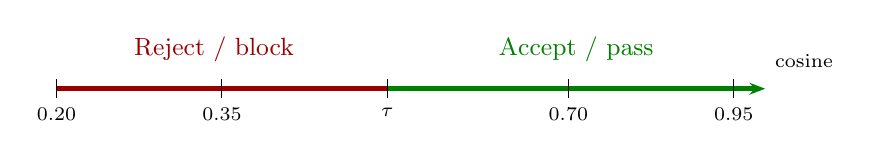
\begin{tikzpicture}[font=\small]
\draw[line width=2pt,red!60!black] (0,0)--(4.2,0);
\draw[line width=2pt,green!50!black,-{Stealth[length=2mm]}] (4.2,0)--(9,0);
\draw (0,0.12)--(0,-0.12) node[below,font=\scriptsize]{0.20};
\draw (2.1,0.12)--(2.1,-0.12) node[below,font=\scriptsize]{0.35};
\draw (4.2,0.12)--(4.2,-0.12) node[below,font=\scriptsize]{$\tau$};
\draw (6.5,0.12)--(6.5,-0.12) node[below,font=\scriptsize]{0.70};
\draw (8.6,0.12)--(8.6,-0.12) node[below,font=\scriptsize]{0.95};
\node[red!60!black] at (2.0,0.5) {Reject / block};
\node[green!50!black] at (6.6,0.5) {Accept / pass};
\node[right,font=\scriptsize] at (9,0.35) {cosine};
\end{tikzpicture}
\caption{SV pass khi $\cos(x,c_{user})\ge\tau$. Runtime dùng $\tau=0.45$ cho ECAPA
own checkpoint (xem \texttt{core/config.py}).}
\end{figure}

% ============================================================
\section{Kết quả và so sánh}
% ============================================================
\begin{figure}[H]
\centering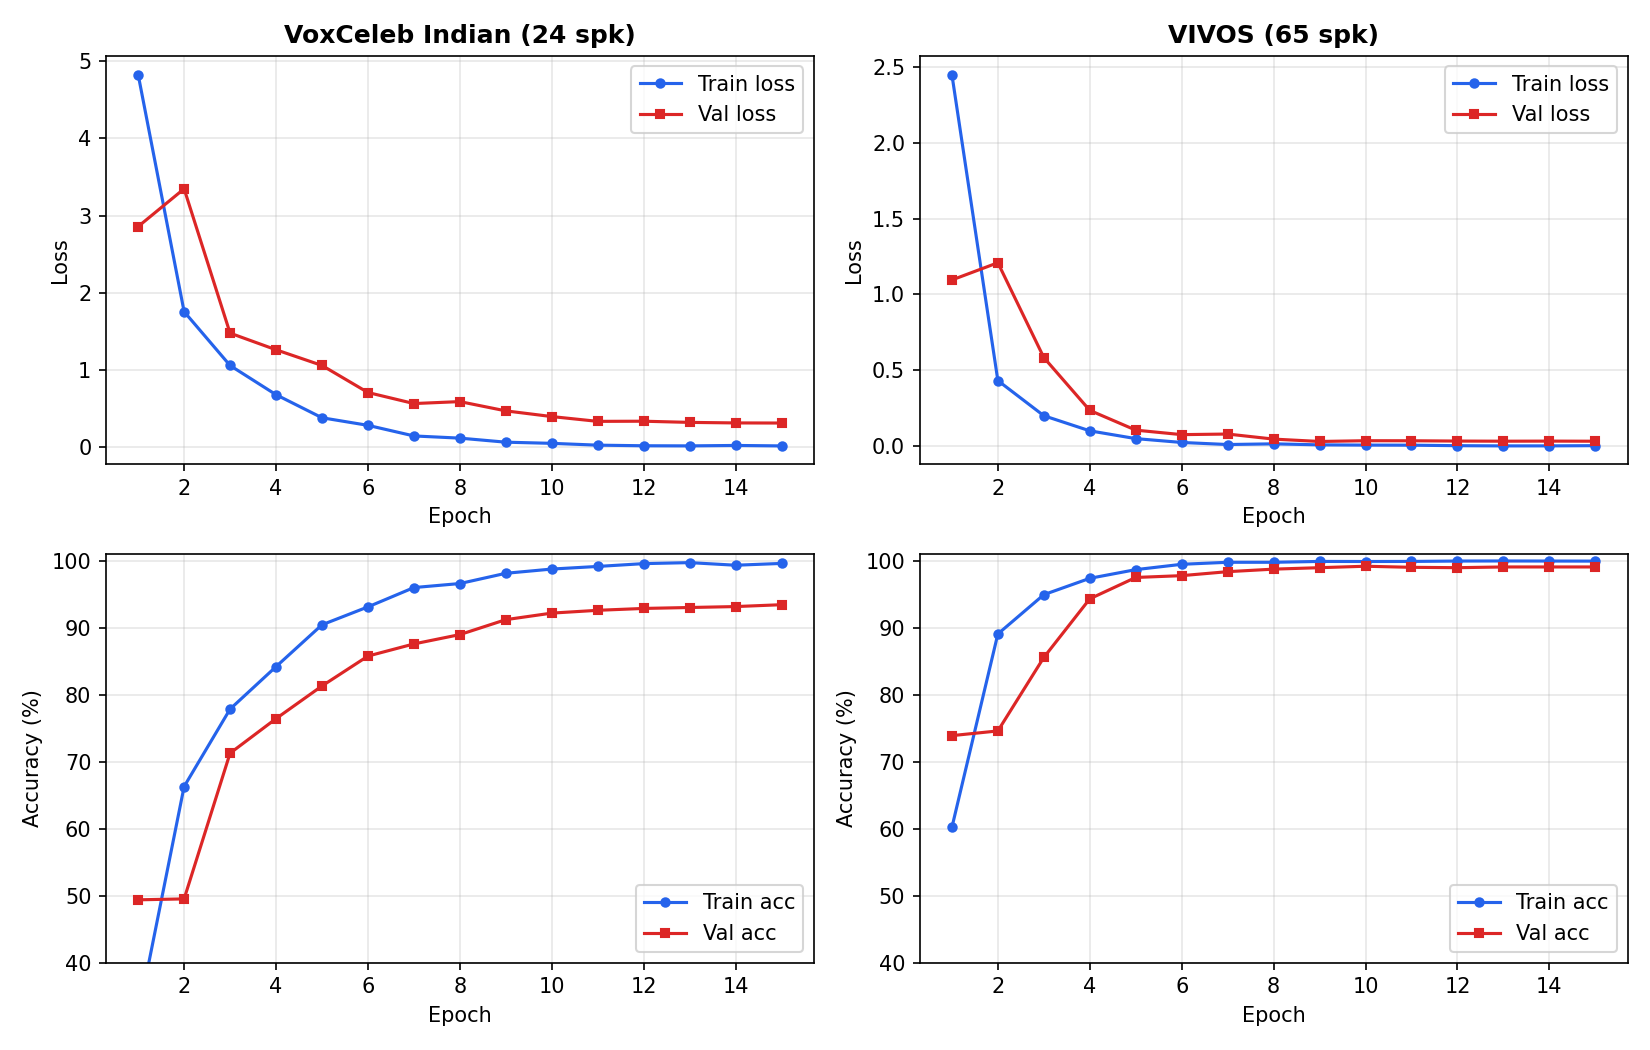
\includegraphics[width=\linewidth]{figs/curves.png}
\caption{Loss (trên) và accuracy (dưới) theo epoch. Hội tụ ổn định, val loss không
bật tăng (không overfit nặng).}
\end{figure}

\begin{figure}[H]
\centering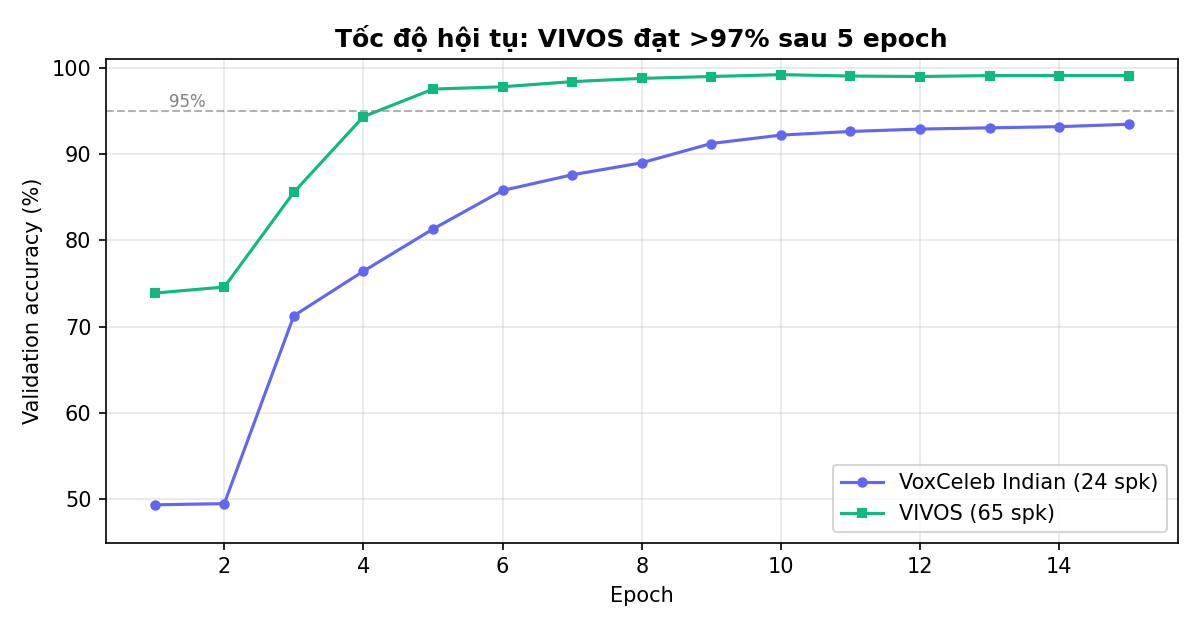
\includegraphics[width=0.78\linewidth]{figs/val_overlay.png}
\caption{So sánh tốc độ hội tụ: VIVOS vượt 97\% val-acc chỉ sau 5 epoch.}
\end{figure}

\begin{table}[H]
\centering\small
\begin{tabular}{lrr}
\toprule
\textbf{Chỉ số} & \textbf{VoxCeleb Indian} & \textbf{VIVOS} \\
\midrule
Best val accuracy & 93.44\% & 99.19\% \\
SID Top-1 / Micro-F1 & 91.34\% & \textbf{99.31\%} \\
SID Top-5 & 98.67\% & \textbf{100.00\%} \\
SID Macro-F1 & \multicolumn{2}{c}{\emph{(cần chạy lại --- Phụ lục~\ref{sec:appendix})}} \\
SV EER & 2.90\% & \textbf{0.96\%} \\
SV minDCF & 0.1486 & \textbf{0.0673} \\
Threshold @ EER & 0.3884 & 0.4062 \\
Số test / trial & 751 / 552 & 1{,}883 / 4{,}160 \\
\bottomrule
\end{tabular}
\caption{Bảng tổng hợp (từ \texttt{sid\_results.json}, \texttt{sv\_results.json}).}
\end{table}

\begin{figure}[H]
\centering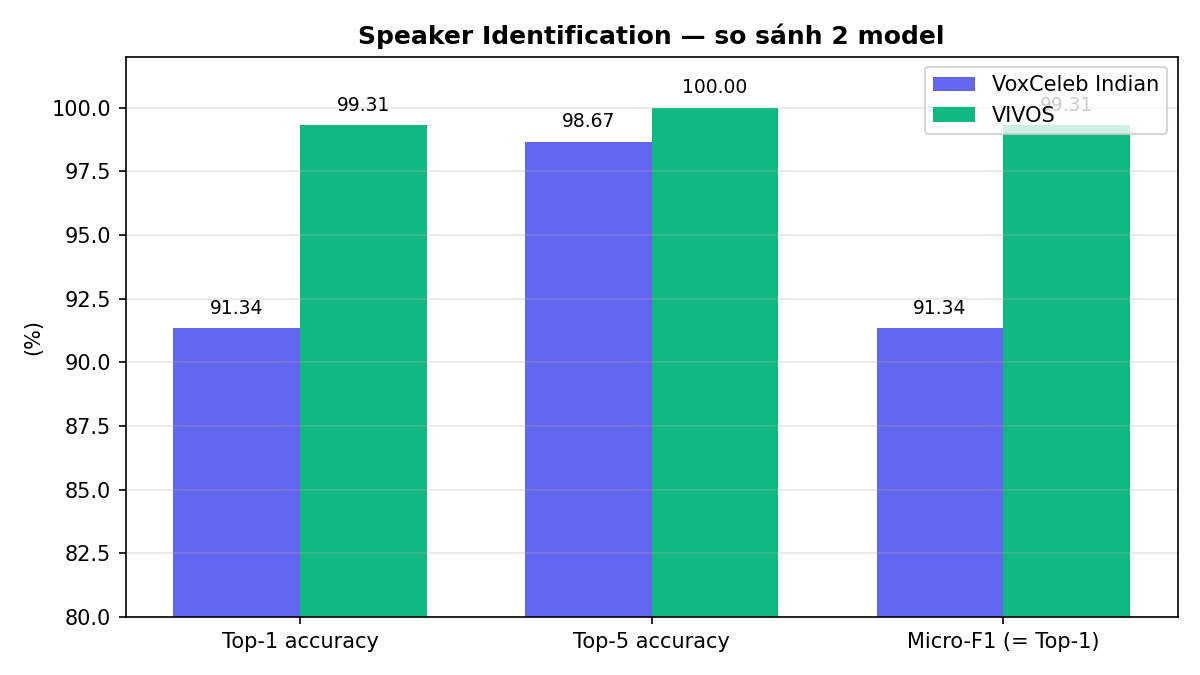
\includegraphics[width=0.84\linewidth]{figs/sid_compare.png}
\caption{So sánh SID. VIVOS gần như hoàn hảo (Top-5 = 100\%).}
\end{figure}
\begin{figure}[H]
\centering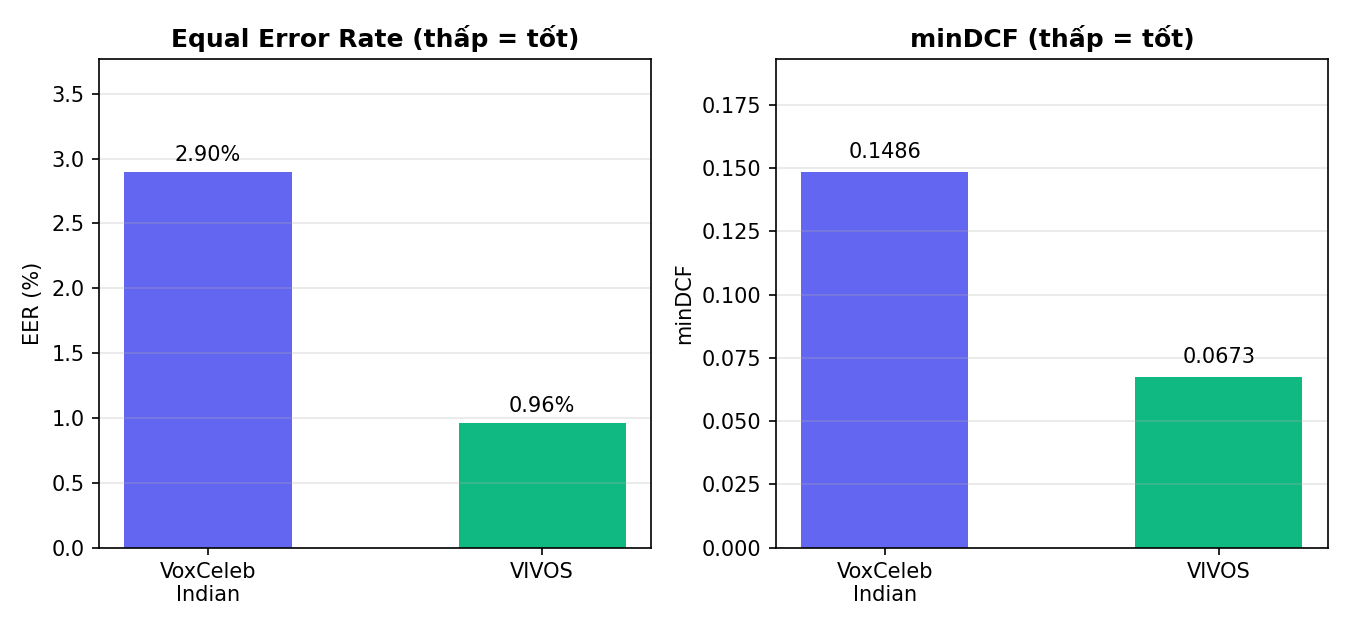
\includegraphics[width=\linewidth]{figs/sv_compare.png}
\caption{So sánh SV (thấp hơn = tốt hơn). VIVOS thấp hơn ở cả EER lẫn minDCF.}
\end{figure}

\subsection{Lịch sử thực nghiệm và độ ổn định (V1/V2/V3)}
\label{sec:variance}
\begin{table}[H]
\centering\small
\begin{tabular}{p{0.05\linewidth}p{0.22\linewidth}p{0.30\linewidth}p{0.32\linewidth}}
\toprule
\textbf{Vòng} & \textbf{Dataset} & \textbf{Thiết lập} & \textbf{Kết quả} \\
\midrule
V1 & VoxCeleb (24) & sơ bộ, 552 trial & Top-1 92.05\%, EER 2.72\%, minDCF 0.1014 \\
V2 & VIVOS (46, chỉ train/waves) & 80/10/10 \emph{không seed}, 20 epoch & Best val 99.56\% (chưa eval) \\
V3 & VoxCeleb (24) \& VIVOS (65) & \textbf{chính thức}, seed=42, 15 epoch & Toàn bộ số ở bảng trên \\
\bottomrule
\end{tabular}
\caption{Ba vòng thực nghiệm; V3 sinh evidence trong \texttt{results/}.}
\end{table}

\begin{diembox}[Bằng chứng run-to-run variance]
So V1 và V3 trên \emph{cùng} VoxCeleb (khác lần xáo trộn): Top-1 $92.05\%\!\to\!91.34\%$,
EER $2.72\%\!\to\!2.90\%$. Mức dao động này \textbf{chứng minh bằng số} cho caveat
``trial set 552 cặp có sai số thống kê''. VIVOS (4{,}160 trial) ổn định hơn nhiều.
\end{diembox}

% ============================================================
\section{Giải thích các file output}
% ============================================================
\begin{table}[H]
\centering\small
\begin{tabular}{p{0.28\linewidth}p{0.65\linewidth}}
\toprule
\textbf{File} & \textbf{Nội dung \& mục đích} \\
\midrule
\texttt{best\_model.pt} & \texttt{state\_dict} của ECAPA + lớp AAM-Softmax, kèm
\texttt{epoch}, \texttt{val\_acc}. File dùng để extract embedding lúc deploy. \\
\texttt{spk2idx.json} & Ánh xạ speaker ID $\to$ chỉ số lớp; bắt buộc giữ để giải mã
dự đoán. \\
\texttt{training\_log.json} & Loss/accuracy train+val theo epoch (vẽ đường cong). \\
\texttt{hparams.json} & Siêu tham số + môi trường (seed, Python, PyTorch, git SHA)
--- phục vụ tái lập. \\
\texttt{sid\_results.json} & Top-1/Top-5 (+ micro/macro/weighted-F1 ở bản nâng cấp). \\
\texttt{sv\_results.json} & EER, threshold, minDCF, số trial. \\
\texttt{iden\_split.txt} & Split: \texttt{<1|2|3> <đường\_dẫn>}. \\
\texttt{veri\_test.txt} & Trial SV: \texttt{<label> <file1> <file2>}. \\
\texttt{dataset\_summary.json} & Thống kê dataset (speaker, utterance, split, trial). \\
\texttt{bad\_audio\_files.txt} & (VIVOS) file lỗi đã loại: \texttt{VIVOSSPK44/train\_VIVOSSPK44\_157.wav}. \\
\bottomrule
\end{tabular}
\caption{Ý nghĩa từng artifact trong \texttt{training/results/<dataset>/}.}
\end{table}

% ============================================================
\section{Lý do chọn mô hình và ưu điểm}
% ============================================================
\textbf{Checkpoint chính cho trợ lý: bản huấn luyện trên VIVOS}
(\texttt{checkpoints/vios/best\_model.pt}).

\begin{diembox}[Làm rõ phạm vi ``cải tiến'']
Hai mô hình dùng \emph{cùng kiến trúc và siêu tham số}; khác biệt là \emph{dữ liệu}.
Vì vậy ưu thế của checkpoint VIVOS so với checkpoint VoxCeleb đến từ phù hợp miền +
chất lượng dữ liệu, không phải thay đổi mạng.
\end{diembox}

\begin{enumerate}
  \item \textbf{Khớp miền tiếng Việt}: người dùng nói tiếng Việt; checkpoint
  VoxCeleb (giọng Ấn) là out-of-domain. VIVOS loại bỏ khoảng cách này.
  \item \textbf{Chính xác hơn ở bài toán khó hơn}: 99.31\% trên 65 người so với
  91.34\% trên 24 người.
  \item \textbf{Xác minh tin cậy hơn}: EER 0.96\% so với 2.90\% ($\sim$3$\times$
  thấp hơn), minDCF 0.0673 so với 0.1486 $\to$ cổng \textsc{Important} an toàn hơn.
  \item \textbf{Thống kê vững hơn}: 4{,}160 trial so với 552.
  \item \textbf{Hội tụ nhanh, ổn định}: val-acc $>$97\% sau 5 epoch.
\end{enumerate}
VoxCeleb Indian vẫn được giữ để \emph{kiểm chứng tính tổng quát} trên dữ liệu nhiễu.

% ============================================================
\section{Hạn chế của phương pháp}
% ============================================================
\begin{enumerate}
  \item Rò rỉ phiên (không group theo \texttt{video\_id}); không phải VoxCeleb1-O.
  \item Trial VoxCeleb nhỏ (552) $\to$ EER nhiễu.
  \item Lệch miền: VIVOS là giọng đọc sạch, dễ hơn thực tế.
  \item Ngưỡng runtime chưa hiệu chỉnh trên người dùng thật.
  \item Chưa bật augmentation trong evidence chính.
  \item SV thuần cosine không chống được replay/voice-clone (cần challenge-response
  ở tầng ứng dụng).
\end{enumerate}

% ============================================================
\section{Hướng cải tiến}
\label{sec:future}
% ============================================================
\begin{enumerate}
  \item \textbf{Chia split theo phiên}: nhóm theo \texttt{video\_id}; dùng bộ trial
  chuẩn VoxCeleb1-O để so sánh với văn liệu.
  \item \textbf{Bật augmentation} (MUSAN + RIR + SpecAugment + speed) --- khung đã
  sẵn --- để tăng độ bền với nhiễu, kỳ vọng giảm EER in-the-wild.
  \item \textbf{Vẽ DET/ROC \& score distribution}: dùng cờ \texttt{-{}-scores-out}
  (vừa thêm vào \texttt{evaluate\_sv.py}) để lưu (label, score), rồi plot đường cong.
  \item \textbf{Confusion matrix \& macro-F1}: chạy \texttt{evaluate\_sid.py}
  \texttt{-{}-confusion-out} (đã thêm), phân tích người nói bị nhầm nhiều nhất.
  \item \textbf{AS-Norm}: chuẩn hoá điểm cosine theo cohort để ngưỡng ổn định giữa
  môi trường (runtime đã có AS-Norm-lite).
  \item \textbf{Khoảng tin cậy EER}: bootstrap trên trial set, đặc biệt cho VoxCeleb.
  \item \textbf{Tăng quy mô \& fine-tune}: pre-train VoxCeleb1+2 rồi fine-tune trên
  tiếng Việt + giọng người dùng.
  \item \textbf{Đo độ trễ \& nén}: ghi nhận latency CPU/GPU, thử quantization để
  triển khai realtime.
  \item \textbf{Anti-spoofing}: thêm mô hình phát hiện replay/synthetic.
\end{enumerate}

% ============================================================
\section{Câu hỏi dự đoán và đáp án}
% ============================================================
\textbf{Câu 1 --- Vì sao chọn ECAPA-TDNN?} Là baseline SOTA cho speaker embedding,
kiểm chứng rộng rãi, có cài đặt SpeechBrain ổn định; SE-Res2Block + attentive
pooling cho embedding tốt với chi phí hợp lý ($\sim$6.2M tham số).

\textbf{Câu 2 --- AAM-Softmax khác Cross-Entropy thường thế nào?} Cộng biên góc
$m=0.2$ vào lớp đúng buộc embedding gần centroid hơn $\to$ inter-class lớn,
intra-class nhỏ trong không gian cosine --- đúng thứ SV/SID cần.

\textbf{Câu 3 --- Vì sao một mô hình dùng cho cả SID và SV?} Train phân loại người
nói tạo embedding phân biệt; SID = argmax cosine, SV = ngưỡng cosine. Không cần hai
mô hình riêng.

\textbf{Câu 4 --- Micro-F1 và Macro-F1 khác gì?} Micro-F1 gộp toàn bộ mẫu $\to$ bằng
accuracy ở bài single-label. Macro-F1 trung bình F1 theo \emph{từng người}, nhạy với
lớp ít mẫu/bị nhầm.

\textbf{Câu 5 --- EER là gì? minDCF là gì?} EER là điểm FAR=FRR (càng thấp càng tốt).
minDCF là chi phí quyết định tối thiểu khi người mục tiêu hiếm ($P_{tar}=0.01$),
khắt khe hơn cho bảo mật.

\textbf{Câu 6 --- Vì sao VIVOS tốt hơn VoxCeleb dù nhiều người hơn?} VIVOS là giọng
đọc sạch, đúng miền tiếng Việt; VoxCeleb Indian là audio YouTube nhiễu, đa kênh, lệch
miền.

\textbf{Câu 7 --- Vì sao random crop khi train, full utterance khi verify?} Random
crop là augmentation thời gian, tăng tổng quát; verify cần embedding ổn định nên
dùng cả câu.

\textbf{Câu 8 --- CMN để làm gì?} Trừ trung bình theo thời gian để khử thiên lệch
kênh/micro $\to$ bền hơn khi đổi thiết bị.

\textbf{Câu 9 --- Train acc gần 100\% có overfit không?} Val loss không bật tăng,
val-acc cao (93--99\%) và checkpoint chọn theo \emph{best val} (early-best) nên
overfit được kiểm soát; tuy vậy caveat rò rỉ phiên khiến số liệu lạc quan hơn thực.

\textbf{Câu 10 --- Vì sao cần margin Top1$-$Top2 (SID) trước SV?} Top-1 cao chưa chắc
tin cậy nếu Top-2 sát; margin nhỏ = mơ hồ giữa hai người. Tầng router chặn trường hợp
ambiguous trước khi xác minh.

% ============================================================
\section{Checklist ôn tập}
% ============================================================
\begin{table}[H]
\centering\small
\begin{tabular}{p{0.04\linewidth}p{0.82\linewidth}p{0.05\linewidth}}
\toprule
\textbf{\#} & \textbf{Nội dung cần nhớ} & \textbf{OK} \\
\midrule
1 & Một embedding ECAPA 192-d dùng cho cả SID (argmax cosine) và SV (ngưỡng cosine). & $\square$ \\
2 & Tiền xử lý: 16kHz $\to$ mono $\to$ crop 3s $\to$ mel 80 + log + CMN. & $\square$ \\
3 & AAM-Softmax (m=0.2, s=30) tạo biên góc $\to$ tách người nói tốt hơn CE. & $\square$ \\
4 & Adam + CosineAnnealingLR + grad clip 5.0; lưu checkpoint best-val. & $\square$ \\
5 & SID: Top-1/Top-5; micro-F1 = Top-1; macro-F1 cần confusion matrix. & $\square$ \\
6 & SV: EER (FAR=FRR), minDCF ($P_{tar}$=0.01); threshold runtime 0.45. & $\square$ \\
7 & VIVOS: 99.31\% Top-1, EER 0.96\% $\to$ checkpoint chính. & $\square$ \\
8 & VoxCeleb: 91.34\%, EER 2.90\%; trial nhỏ $\to$ EER nhiễu (V1 vs V3). & $\square$ \\
9 & Caveat: rò rỉ phiên, lệch miền, chưa augment. & $\square$ \\
10 & Cải tiến: group-split, augmentation, DET curve, macro-F1, AS-Norm. & $\square$ \\
\bottomrule
\end{tabular}
\end{table}

% ============================================================
\section{Tóm tắt một đoạn để nói}
% ============================================================
YC1 huấn luyện một mô hình ECAPA-TDNN sinh embedding 192 chiều phục vụ cả nhận diện
(SID) lẫn xác minh người nói (SV). Audio được đưa về 16kHz mono, cắt 3 giây, trích
mel-filterbank 80 chiều rồi log + CMN; mạng được train bằng AAM-Softmax (biên góc
0.2, scale 30) với Adam + cosine LR + gradient clipping, lưu checkpoint theo val
accuracy cao nhất. SID đo Top-1/Top-5 (micro-F1 = Top-1), SV đo EER và minDCF bằng
cosine similarity giữa các embedding. Trên VIVOS, mô hình đạt Top-1 99.31\% và EER
0.96\%, vượt trội checkpoint VoxCeleb Indian (91.34\%, 2.90\%) chủ yếu nhờ khớp miền
tiếng Việt và dữ liệu sạch --- nên VIVOS được chọn làm checkpoint chính. Các hạn chế
(rò rỉ phiên, trial nhỏ, chưa augment) và hướng cải tiến (group-split, augmentation,
DET curve, macro-F1, AS-Norm) đều được nêu rõ.

% ============================================================
\section{Gợi ý thứ tự trình bày 5 phút}
% ============================================================
\begin{enumerate}
  \item \textbf{30s} --- Bài toán: SID vs SV, vì sao một embedding dùng cho cả hai.
  \item \textbf{60s} --- Tiền xử lý + mel + CMN (sơ đồ pipeline).
  \item \textbf{60s} --- ECAPA-TDNN + AAM-Softmax (vì sao biên góc).
  \item \textbf{60s} --- Đánh giá: Top-1/F1, EER, minDCF (đường cong + bảng).
  \item \textbf{60s} --- So sánh VoxCeleb vs VIVOS, lý do chọn VIVOS.
  \item \textbf{30s} --- Caveat + hướng cải tiến.
\end{enumerate}

% ============================================================
\section{Kết luận}
% ============================================================
Phần YC1 xây dựng lõi sinh trắc giọng nói: một mô hình ECAPA-TDNN, train bằng
AAM-Softmax, dùng cosine similarity cho cả SID và SV. Quy trình từ tiền xử lý, kiến
trúc, huấn luyện đến đánh giá đều được kiểm soát và tái lập (seed, hparams), với
evidence thật trên hai dataset. Checkpoint VIVOS được chọn nhờ khớp miền tiếng Việt
và chỉ số tốt nhất. Báo cáo trình bày trung thực cả điểm mạnh lẫn hạn chế, và để
sẵn các móc nối kỹ thuật (cờ \texttt{-{}-scores-out}, \texttt{-{}-confusion-out},
khung augmentation) cho các cải tiến tiếp theo.

% ============================================================
\section{Phụ lục: lệnh tái lập}
\label{sec:appendix}
% ============================================================
\begin{lstlisting}[language=bash]
# Train
python train_ecapa.py --data_root <data> --split_file <iden_split.txt> \
    --save_dir results/<dataset> --epochs 15 --batch_size 64 --lr 1e-3

# Danh gia SID (da co macro-F1 + confusion matrix)
python evaluate_sid.py --ckpt results/<dataset>/best_model.pt \
    --spk2idx results/<dataset>/spk2idx.json \
    --data_root <data> --split_file <iden_split.txt> \
    --out results/<dataset>/sid_results.json \
    --confusion-out results/<dataset>/confusion.json

# Danh gia SV (luu them scores de ve DET/ROC)
python evaluate_sv.py --ckpt results/<dataset>/best_model.pt \
    --data_root <data> --trial_file <veri_test.txt> \
    --out results/<dataset>/sv_results.json \
    --scores-out results/<dataset>/sv_scores.json
\end{lstlisting}

\vfill
\noindent\rule{\linewidth}{0.4pt}\\
\small Nguồn: \texttt{training/train\_ecapa.py}, \texttt{evaluate\_sid.py},
\texttt{evaluate\_sv.py}, \texttt{augmentations.py}, \texttt{notebooks/SecureVA-V3.ipynb}
và \texttt{training/results/}. Biểu đồ tạo bằng \texttt{training/report/make\_figures.py}.
Kiến trúc: Desplanques et al., \emph{ECAPA-TDNN}, Interspeech 2020; SpeechBrain.

\end{document}
